\documentclass[11pt]{article}

\usepackage{url}
\usepackage{multicol}
\usepackage[english]{babel}
\usepackage[margin=1in]{geometry}
\usepackage{graphicx}
\usepackage{subcaption}
\usepackage{enumitem}
\usepackage{amsmath}
\usepackage{amssymb}
\usepackage{wasysym}
\usepackage{color}
\usepackage{float}
\usepackage{nomencl}
\usepackage[title]{appendix}
\makenomenclature
\usepackage{pdfpages}
\usepackage{algorithm}
\usepackage{algpseudocode}
\usepackage{hyperref}
\hypersetup{
    colorlinks=true,
    linkcolor=blue,
    filecolor=magenta,      
    urlcolor=cyan,
    pdftitle={Overleaf Example},
    pdfpagemode=FullScreen,
    }
\title{16-745 Optimal Control Lecture 2}
\author{Reid Graves} 

\begin{document}
\maketitle

\section{Last time}
\begin{itemize}
    \item Continuous Time Dynamics
    \item Manipulator Dynamics
    \item Linear Systems
\end{itemize}
Won't need to derive these for this class.

\section{Today}
\begin{itemize}
    \item Equilibria
    \item Stability
    \item Discrete Time Dynamics and Simulation
\end{itemize}

\section{Equilibria}
\begin{itemize}
    \item A point where the system will "remain at rest"
    \begin{align*}
        \dot{x} &= f(x,u) = 0
    \end{align*}
    \item Algebraically, roots of the dynamics
    \item Look at Pendulum again
    \begin{align*}
        \dot{x} &= \begin{bmatrix}
            \dot{\theta} \\
            \frac{-q}{l}\sin(\theta)
        \end{bmatrix}
        =
        \begin{bmatrix}
            0 \\
            0
        \end{bmatrix}
        \\
        \dot{\theta} &= 0
        \\
        \theta &= 0,\pi
    \end{align*}
    \begin{figure}[H]
        \centering
        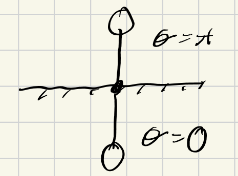
\includegraphics[width=0.4\linewidth]{lecture_2_1.png}
        \caption{Pendulum}
        \label{pendulum1}
    \end{figure}
\end{itemize}
\subsection{First control Problem}
\begin{itemize}
    \item Can I move the equilibria?
    \begin{figure}[H]
        \centering
        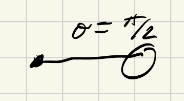
\includegraphics[width=0.4\linewidth]{lecture_2_2.png}
        \caption{Moving pendulum equilibria}
        \label{pendulum2}
    \end{figure}
    \begin{align*}
        \theta &= \frac{\pi}{2} & \dot{x} &= \begin{bmatrix}
            \dot{\theta} \\
            \frac{-q}{l}\sin\left(\frac{\pi}{2}\right) + \frac{1}{ml^2}u
        \end{bmatrix}
        =
        \begin{bmatrix}
            0 \\
            0
        \end{bmatrix}
        \\
        \frac{1}{ml^2}u &= \frac{q}{l}\sin\left(\frac{\pi}{2}\right)
        \\
        u &= mgl
    \end{align*}
    \item In general, we get a root finding problem in u:
    \begin{align*}
        f(x^*,u) &= 0
    \end{align*}
\end{itemize}

\section{Stability of Equilibria}
\begin{itemize}
    \item When will we stay "near" an equilibrium point under perturbations?
    \item Look at a 1D system (1 dimensional state space) $x\in \mathbb{R}$
    % Insert plot here
    \begin{figure}[H]
        \centering
        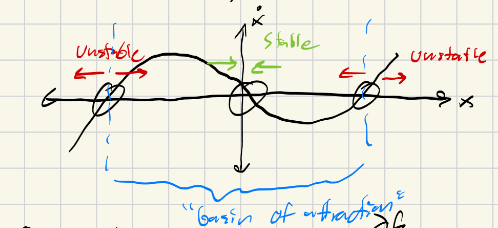
\includegraphics[width=0.5\linewidth]{lecture_2_3.png}
        \caption{Stability at equilibria graphic}
        \label{plot3}
    \end{figure}
    \item If $\frac{df}{dx}<0$, stable
    \item If $\frac{df}{dx}>0$, unstable
    \item Basin of attraction: area between the two unstable points
    \item In higher dimensions: $\frac{\partial f}{\partial x}$ is a Jacobian Matrix
    \item Take an Eigendecomposition $\rightarrow$ Decouple into $n$ 1D systems
    \begin{align*}
        Re\left[eigvals\left(\frac{\partial f}{\partial x}\right)\right] < 0 \rightarrow \text{stable}
    \end{align*}
    Otherwise $\rightarrow$ Unstable
    \item Pendulum:
    \begin{align*}
        f(x) &= \begin{bmatrix}
            \dot{\theta} \\
            \frac{-q}{l}\sin(\theta)
        \end{bmatrix}
        \rightarrow
        \frac{\partial f}{\partial x} = \begin{bmatrix}
            0 & 1 \\
            \frac{-q}{l}\cos(\theta) & 0
        \end{bmatrix}
        \\
        \frac{\partial f}{\partial x}|_{\theta=\pi} &= \begin{bmatrix}
            0 & 1 \\
            \frac{q}{l} & 0
        \end{bmatrix}
        \\
        eigvals = \pm \sqrt{\frac{q}{l}}\rightarrow\text{unstable}
    \end{align*}
    \begin{align*}
        \frac{\partial f}{\partial x}_{\theta = 0} &= \begin{bmatrix}
            0 & 1 \\
            \frac{-q}{l} & 0
        \end{bmatrix}
        \rightarrow \text{eigvals} = \pm i\sqrt{\frac{q}{l}}
        \\
        \rightarrow\text{Undamped oscillation}
    \end{align*}
    \item Add damping (e.g. $u=-kd\dot{\theta}$) results in strictly negative real part
\end{itemize}

\section{Discrete Time Dynamics}
\begin{itemize}
    \item Motivation:
    \begin{itemize}
        \item In general, we can't solve $\dot{x}=f(x)$ for $x(t)$
        \item Computationally, need to represent $x(t)$ with a set of discrete $x_k$
        \item Discrete-time models can capture some effects that continuous ODEs can't (like a brick hitting the ground)
    \end{itemize}
    \item Explicit Form:
    \begin{align*}
        x_{k+1} &= f_d(x_k,u_k)
    \end{align*}
    \item Simplest discretization:
    \begin{align*}
        x_{k+1} &= x_k + hf(x_k,u_k)
    \end{align*}
    $h$ is time step, whole right hand side is $f_d(x_k,u_k)$. Whole thing is called \textbf{Forward Euler Integration}
    \item Forward Euler integration adds energy- If you have an oscillatory system, this method always adds energy, causing the system to explode
    \item Pendulum Sim:
    \begin{align*}
        l &= m = 1 
    \end{align*}
\end{itemize}

\subsection{Stability of discrete time systems}
\begin{itemize}
    \item In discrete time, dynamics is an iterated map:
    \begin{align*}
        x_n &= f_d(f_d(f_d(f_d\dots f_d(x_0))))
    \end{align*}
    \item Linearize and apply chain rule:
    \begin{align*}
        \frac{\partial x_k}{\operatorname{x_0}} &= \frac{\partial f_d}{x}|_{x_0}\frac{\partial f_d}{x}|_{x_0} \dots \frac{\partial f_d}{x}|_{x_0} = A_d^N
    \end{align*}
    \item Assume $x_0 = 0$ is an equilibrium
    \begin{align*}
        \text{stable} \rightarrow \lim_{k\rightarrow \infty} A_d^kx_0 &= 0\quad \forall x_0
        \\
        \rightarrow \lim_{k\rightarrow\infty} A_d^k &= 0
        \\
        \rightarrow |eigvals(A_d)| < 1 & \text{    (Inside unit circle)}
    \end{align*}
    \item Pendulum with Forward Euler:
    \begin{align*}
        x_{k+1} &= x_k + hf(x_k)
    \end{align*}
    Right side is $f_d(x_k)$
    \begin{align*}
        Ad &= \frac{\partial f_d}{\partial x} &= I + HA &= I + h\begin{bmatrix}
            0 & 1 \\
            \frac{-q}{l}\cos(\theta) & 0
        \end{bmatrix}
        \\
        eigvals(A_d|_{\theta\approx 0})
    \end{align*}
    \item Key takeaway: \textbf{Never Use Forward Euler}
    \item Intuition:
    % insert figure here
    \begin{figure}[H]
        \centering
        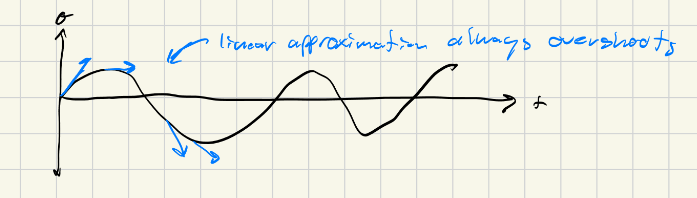
\includegraphics[width=0.75\linewidth]{lecture_2_4.png}
        \caption{Linear approximator always overshoots}
        \label{plot4}
    \end{figure}
    Linear Approximation always overshoots
    \item Take Aways:
    \begin{itemize}
        \item Be careful
        \item Always sanity check e.g. energy, momentum behavior
        \item Never use forward Euler!
    \end{itemize}
    \item A better explicit integrator:
    \begin{itemize}
        \item 4th order Runge-Kutta Method
        \item RK4 fits a cubic polynomial to $x(t)$ rather than a line- Much better accuracy!
        \item Pseudo Code:
        \begin{align*}
            x_{k+1} &= f_d(x_k)
            \\
            k_1 &= f(x_k)
            \\
            k_2 &= f(x_k + \frac{h}{2}k_1)
            \\
            k_3 &= f(x_k + \frac{h}{2}k_2)
            \\
            k_4 &= f(x_k + h k_3
            \\
            x_{x+1} &= x_k + \frac{h}{6}(k_1 + 2k_2 + 2k_3 + k_4)
        \end{align*}
    \end{itemize}
    \item take away:
    \begin{itemize}
        \item Accuracy $>>$ additional compute cost
        \item Even "good" integrators have issues
        \item Always sanity check
    \end{itemize}
\end{itemize}






\end{document}
